\documentclass{article}
\usepackage{pgfplots}
\pgfplotsset{compat=1.18}

\begin{document}

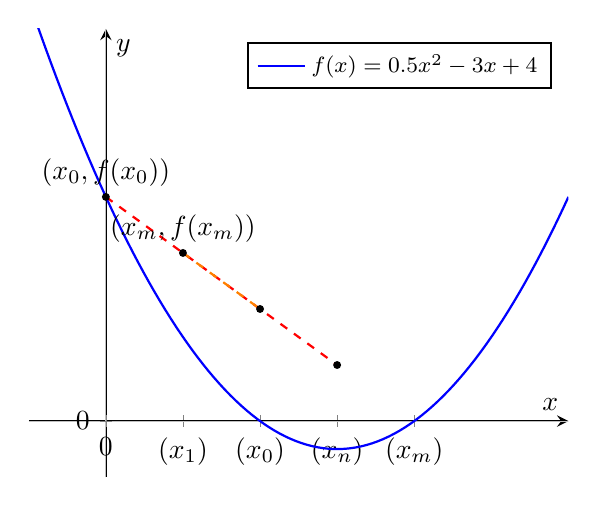
\begin{tikzpicture}
    \begin{axis}[
        axis lines=middle,
        xlabel=$x$,
        ylabel=$y$,
        xmin=-1, xmax=6,
        ymin=-1, ymax=7,
        xtick={0,1,2,3,4},
        ytick={0},
        xticklabels={$x_0$, $(x_1)$, $(x_0)$, $(x_n)$, $(x_m)$},
        yticklabels={$0$},
        extra x ticks={0},
        extra x tick labels={$0$},
        extra y ticks={0},
        extra y tick labels={$0$},
        extra tick style={grid=major},
        domain=-1:6,
        samples=100,
        no markers,
        thick,
        legend pos=north east,
        legend cell align=left,
        legend style={font=\footnotesize},
    ]
    
    % Plot the function f(x) = 0.5x^2 - 3x + 4
    \addplot [blue] {0.5*x^2 - 3*x + 4};
    
    % Plot the tangent line at x_0
    \addplot [red, dashed] coordinates {(0,4) (3,1)};
    
    % Plot the tangent line at x_m
    \addplot [orange, dashed] coordinates {(1,3) (2,2)};
    
    % Markers for the points
    \filldraw [black] (0,4) circle (1pt) node[anchor=south] {$(x_0,f(x_0))$};
    \filldraw [black] (1,3) circle (1pt) node[anchor=south] {$(x_m,f(x_m))$};
    \filldraw [black] (2,2) circle (1pt);
    \filldraw [black] (3,1) circle (1pt);
    
    % Legend
    \legend{$f(x)=0.5x^2-3x+4$};
    
\end{axis}
\end{tikzpicture}

\begin{center}
\textbf{Illustration of Newton's method in 1 variable case, aiming to find the root of the nonlinear equation $f(x) = 0.5x^2 - 3x + 4$. First we initialize the guessed solution $x_0$. The tangent line to $f(x)$ at $x_0$ intersects the $x$-axis at the point $x_1$, which is the updated solution. The procedure is then iterated multiple times until the real root is found, or at least a desired approximation is reached. We note that since the equation might have more than 1 solution, the initialization is critical as the method would drive toward the closest root. On the same figure, we can see that if initially we begin at $x_m$ (on the left), then we end up with different root.}
\end{center}

\end{document}